\documentclass{beamer}
\usepackage{listings}
\usepackage{graphicx}

\graphicspath{{./res/}}

\usepackage{xcolor}

\definecolor{codegreen}{rgb}{0,0.6,0}
\definecolor{codegray}{rgb}{0.5,0.5,0.5}
\definecolor{codepurple}{rgb}{0.58,0,0.82}
\definecolor{backcolour}{rgb}{0.95,0.95,0.92}

\lstdefinestyle{mystyle}{
    language=C,
    morekeywords={MPI_Send, MPI_Recv, MPI_COMM_WORLD, MPI_DOUBLE, MPI_Init, MPI_Finalize, MPI_Comm_rank, MPI_Comm_size},
    backgroundcolor=\color{backcolour},   
    commentstyle=\color{codegreen},
    keywordstyle=\color{magenta},
    numberstyle=\tiny\color{codegray},
    stringstyle=\color{codepurple},
    basicstyle=\ttfamily\footnotesize,
    breakatwhitespace=false,         
    breaklines=true,                 
    captionpos=b,                    
    keepspaces=true,                 
    numbers=left,                    
    numbersep=5pt,                  
    showspaces=false,                
    showstringspaces=false,
    showtabs=false,                  
    tabsize=2
}

\lstset{style=mystyle}

\AtBeginSection[]
{
  \begin{frame}
    \frametitle{}
    \tableofcontents[currentsection]
  \end{frame}
}

\addtobeamertemplate{navigation symbols}{}{%
    \usebeamerfont{footline}%
    \usebeamercolor[fg]{footline}%
    \hspace{1em}%
    \insertframenumber/\inserttotalframenumber
}
\setbeamercolor{footline}{fg=blue}
\setbeamerfont{footline}{series=\bfseries}



\title[]{HPC Project}

\subtitle{CISD}

\author[Marques, Paillé, Chollon, Jonquière]
{L. Marques \and L. Paillé \and M. Chollon \and V. Jonquière}

\date[]
{\today}

\begin{document}

\frame{\titlepage}

\begin{frame}
\frametitle{Table of Contents}
\tableofcontents
\end{frame}

\section{MPI GEMM}

\subsection{Implementation}
\begin{frame}
\frametitle{Main ideas}
\begin{itemize}
    \item Code will run on multiple nodes
    \item Matrices will not be fully loaded on each nodes
\end{itemize}
\end{frame}

\begin{frame}[fragile]
    \frametitle{Base code}
    \textit{Code from dgemm\_tiled\_mpi.c}
    \begin{lstlisting}[language=C]
       double wsA[b * b], wsB[b * b];
       ...
        if (global_options.mpirank == ownerA)
        {
            MPI_Send(A[MT * k + m], b * kk,
                    MPI_DOUBLE, ownerC, MT * k + m,
                    MPI_COMM_WORLD);
        }
        ...
        dgemm_seq(CblasColMajor, transA, transB,
                    mm, nn, kk,
                    alpha, Aptr, b, Bptr, b,
                    lbeta, C[MT * n + m], b);

       
    \end{lstlisting}
\end{frame}


\subsection{Results}
\begin{frame}
\frametitle{SUMMA}
\begin{itemize}
    \item Scalable Universal Matrix Multiplication Algorithm
    \item Solves multiple issues (uses collective communications, workspaces dynamicaly allocated)
\end{itemize}
\end{frame}

\begin{frame}
\frametitle{SUMMA}
\begin{figure}
    \centering
    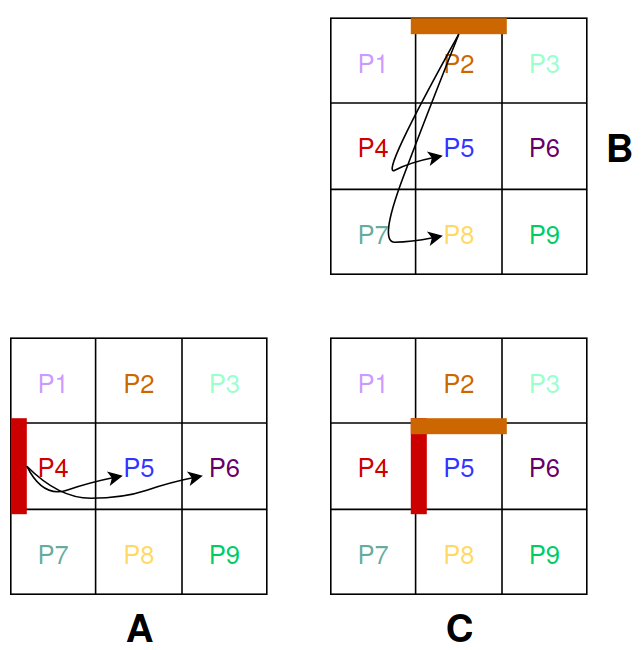
\includegraphics[width=7cm]{SUMMA.png}
    \caption{SUMMA algorithm schema}
\end{figure}
\end{frame}


\begin{frame}
\frametitle{Comparison with OpenMP}
\begin{figure}
    \centering
    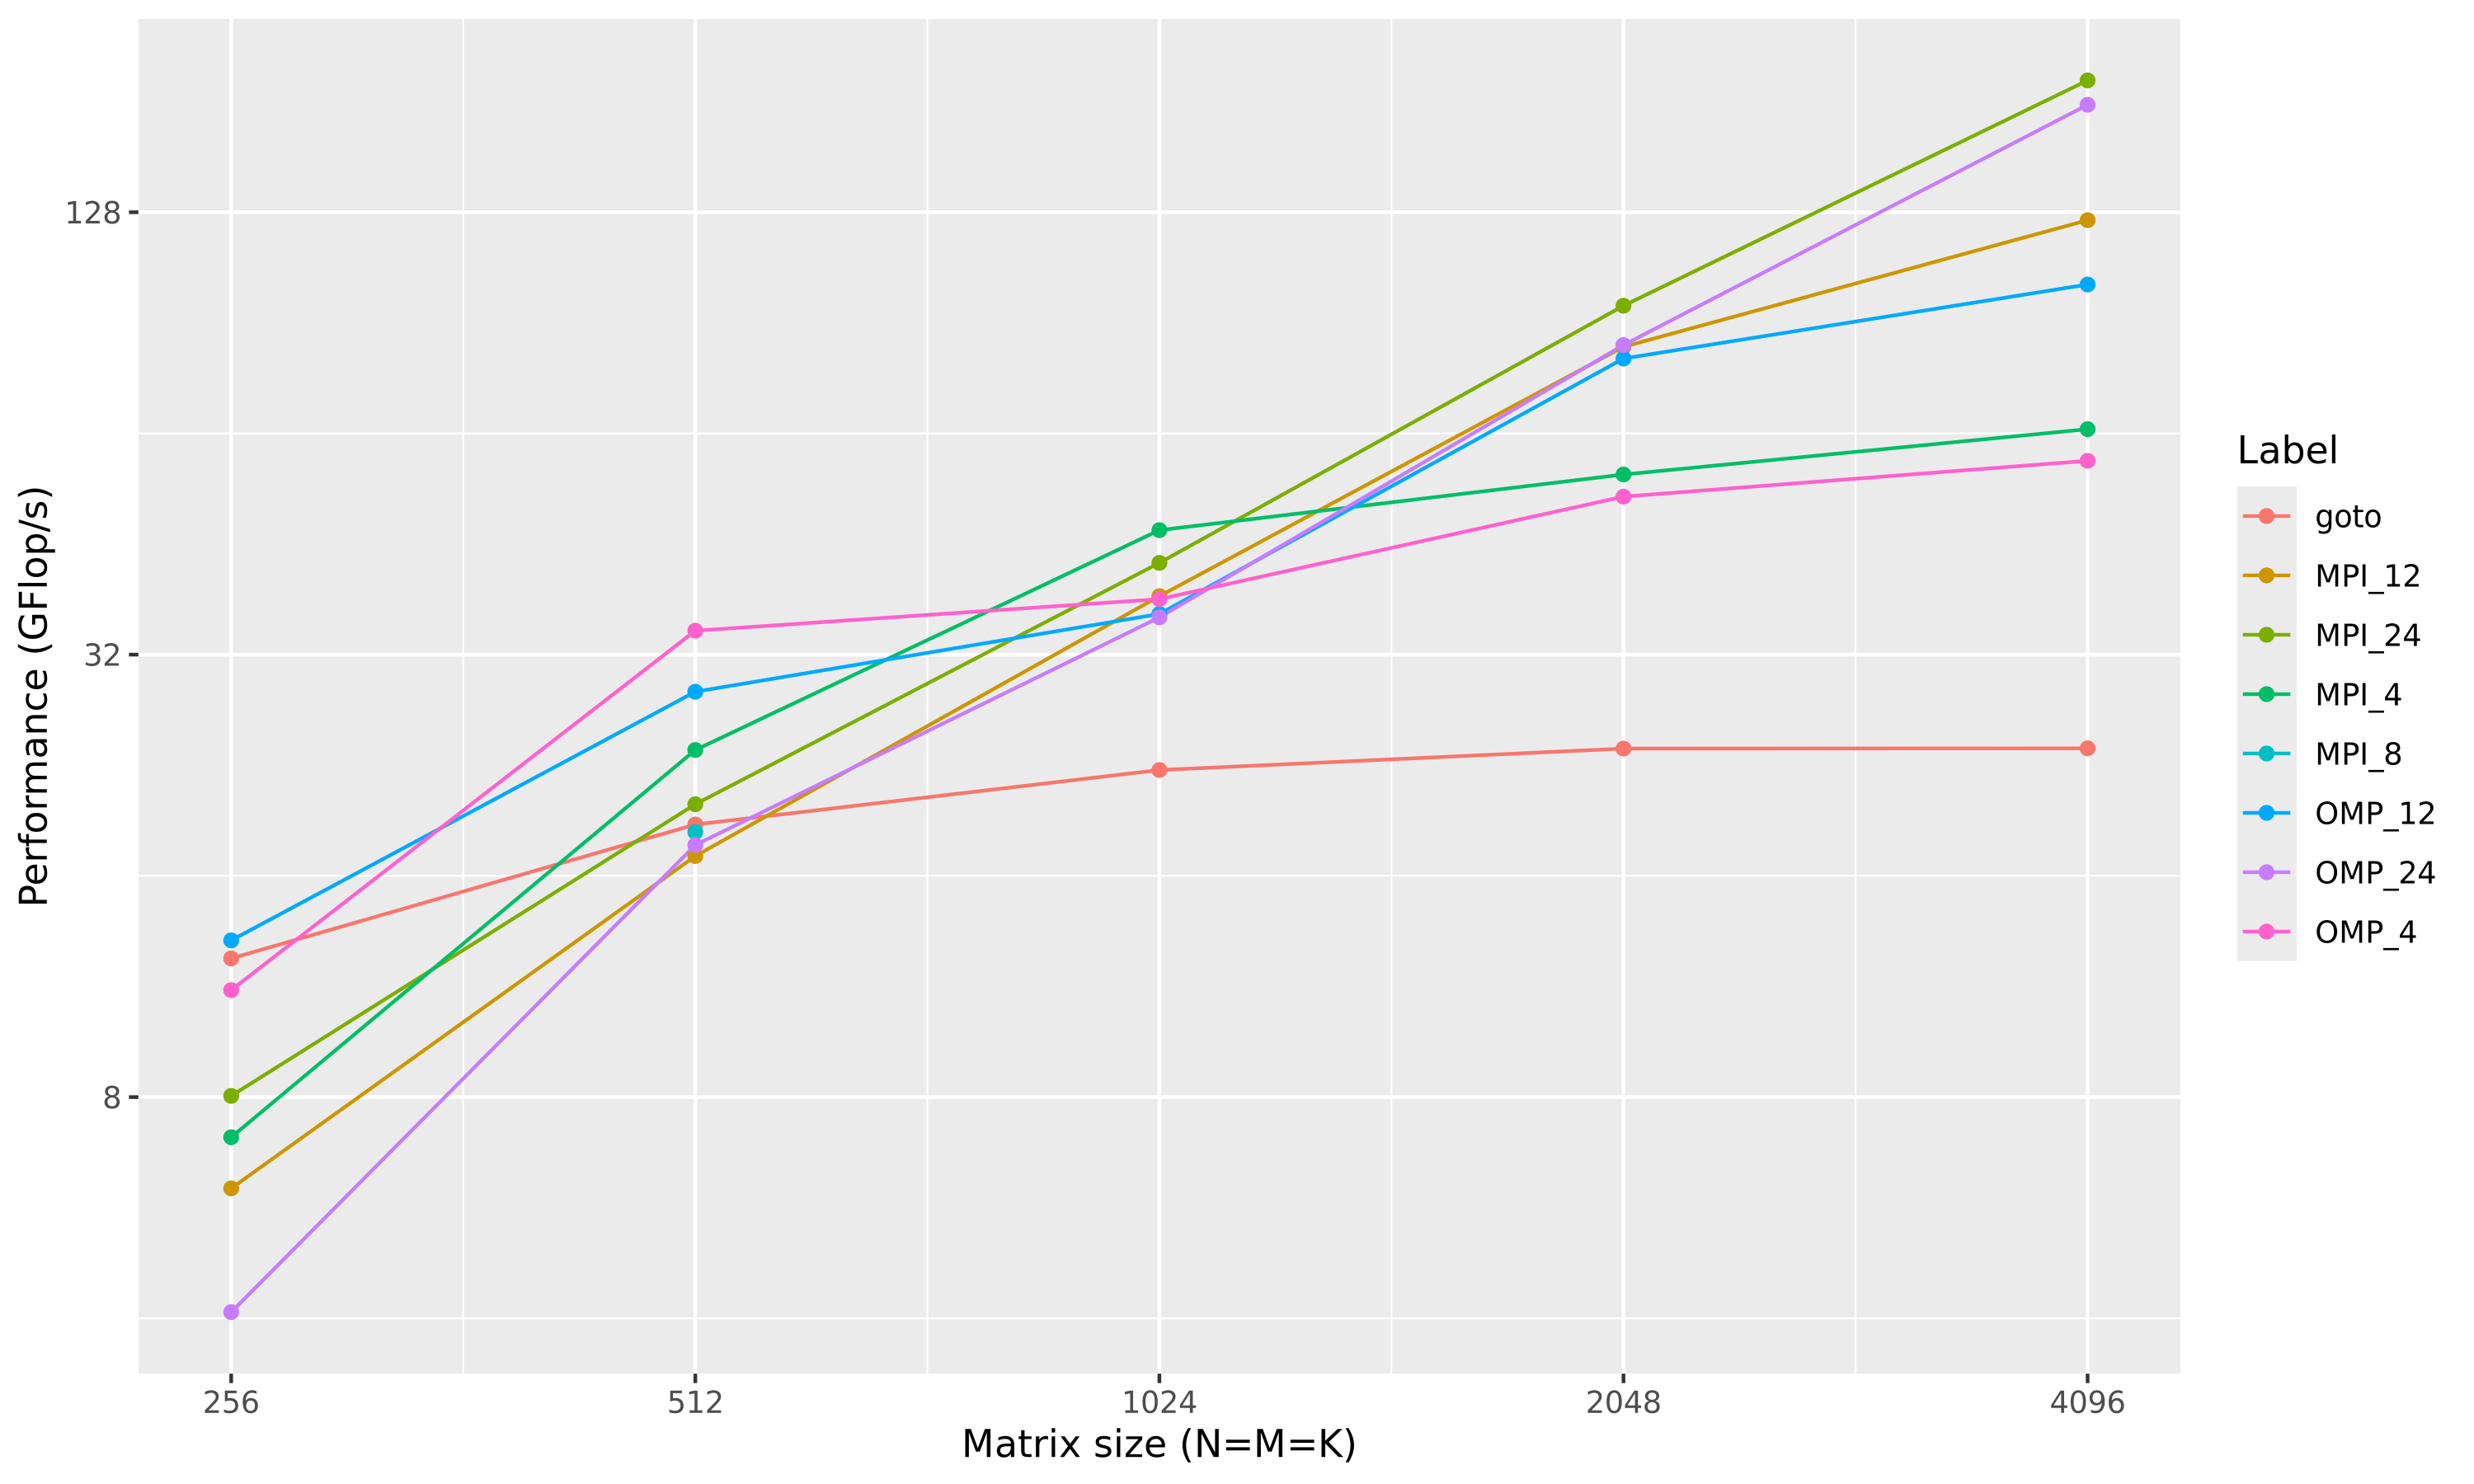
\includegraphics[width=\textwidth]{MPI_vs_OMP.png}
    \caption{Performance depending on number of threads/processes}
\end{figure}

\end{frame}

\begin{frame}
\frametitle{Find the best parameters}
As our algorithm uses shared memory, several (new) parameters needs to be optimized:
\begin{itemize}
    \item Number of nodes
    \item Number of threads/processes per nodes
    \item Block size
\end{itemize}
\end{frame}

\begin{frame}
\frametitle{Block size}
\begin{figure}
    \centering
    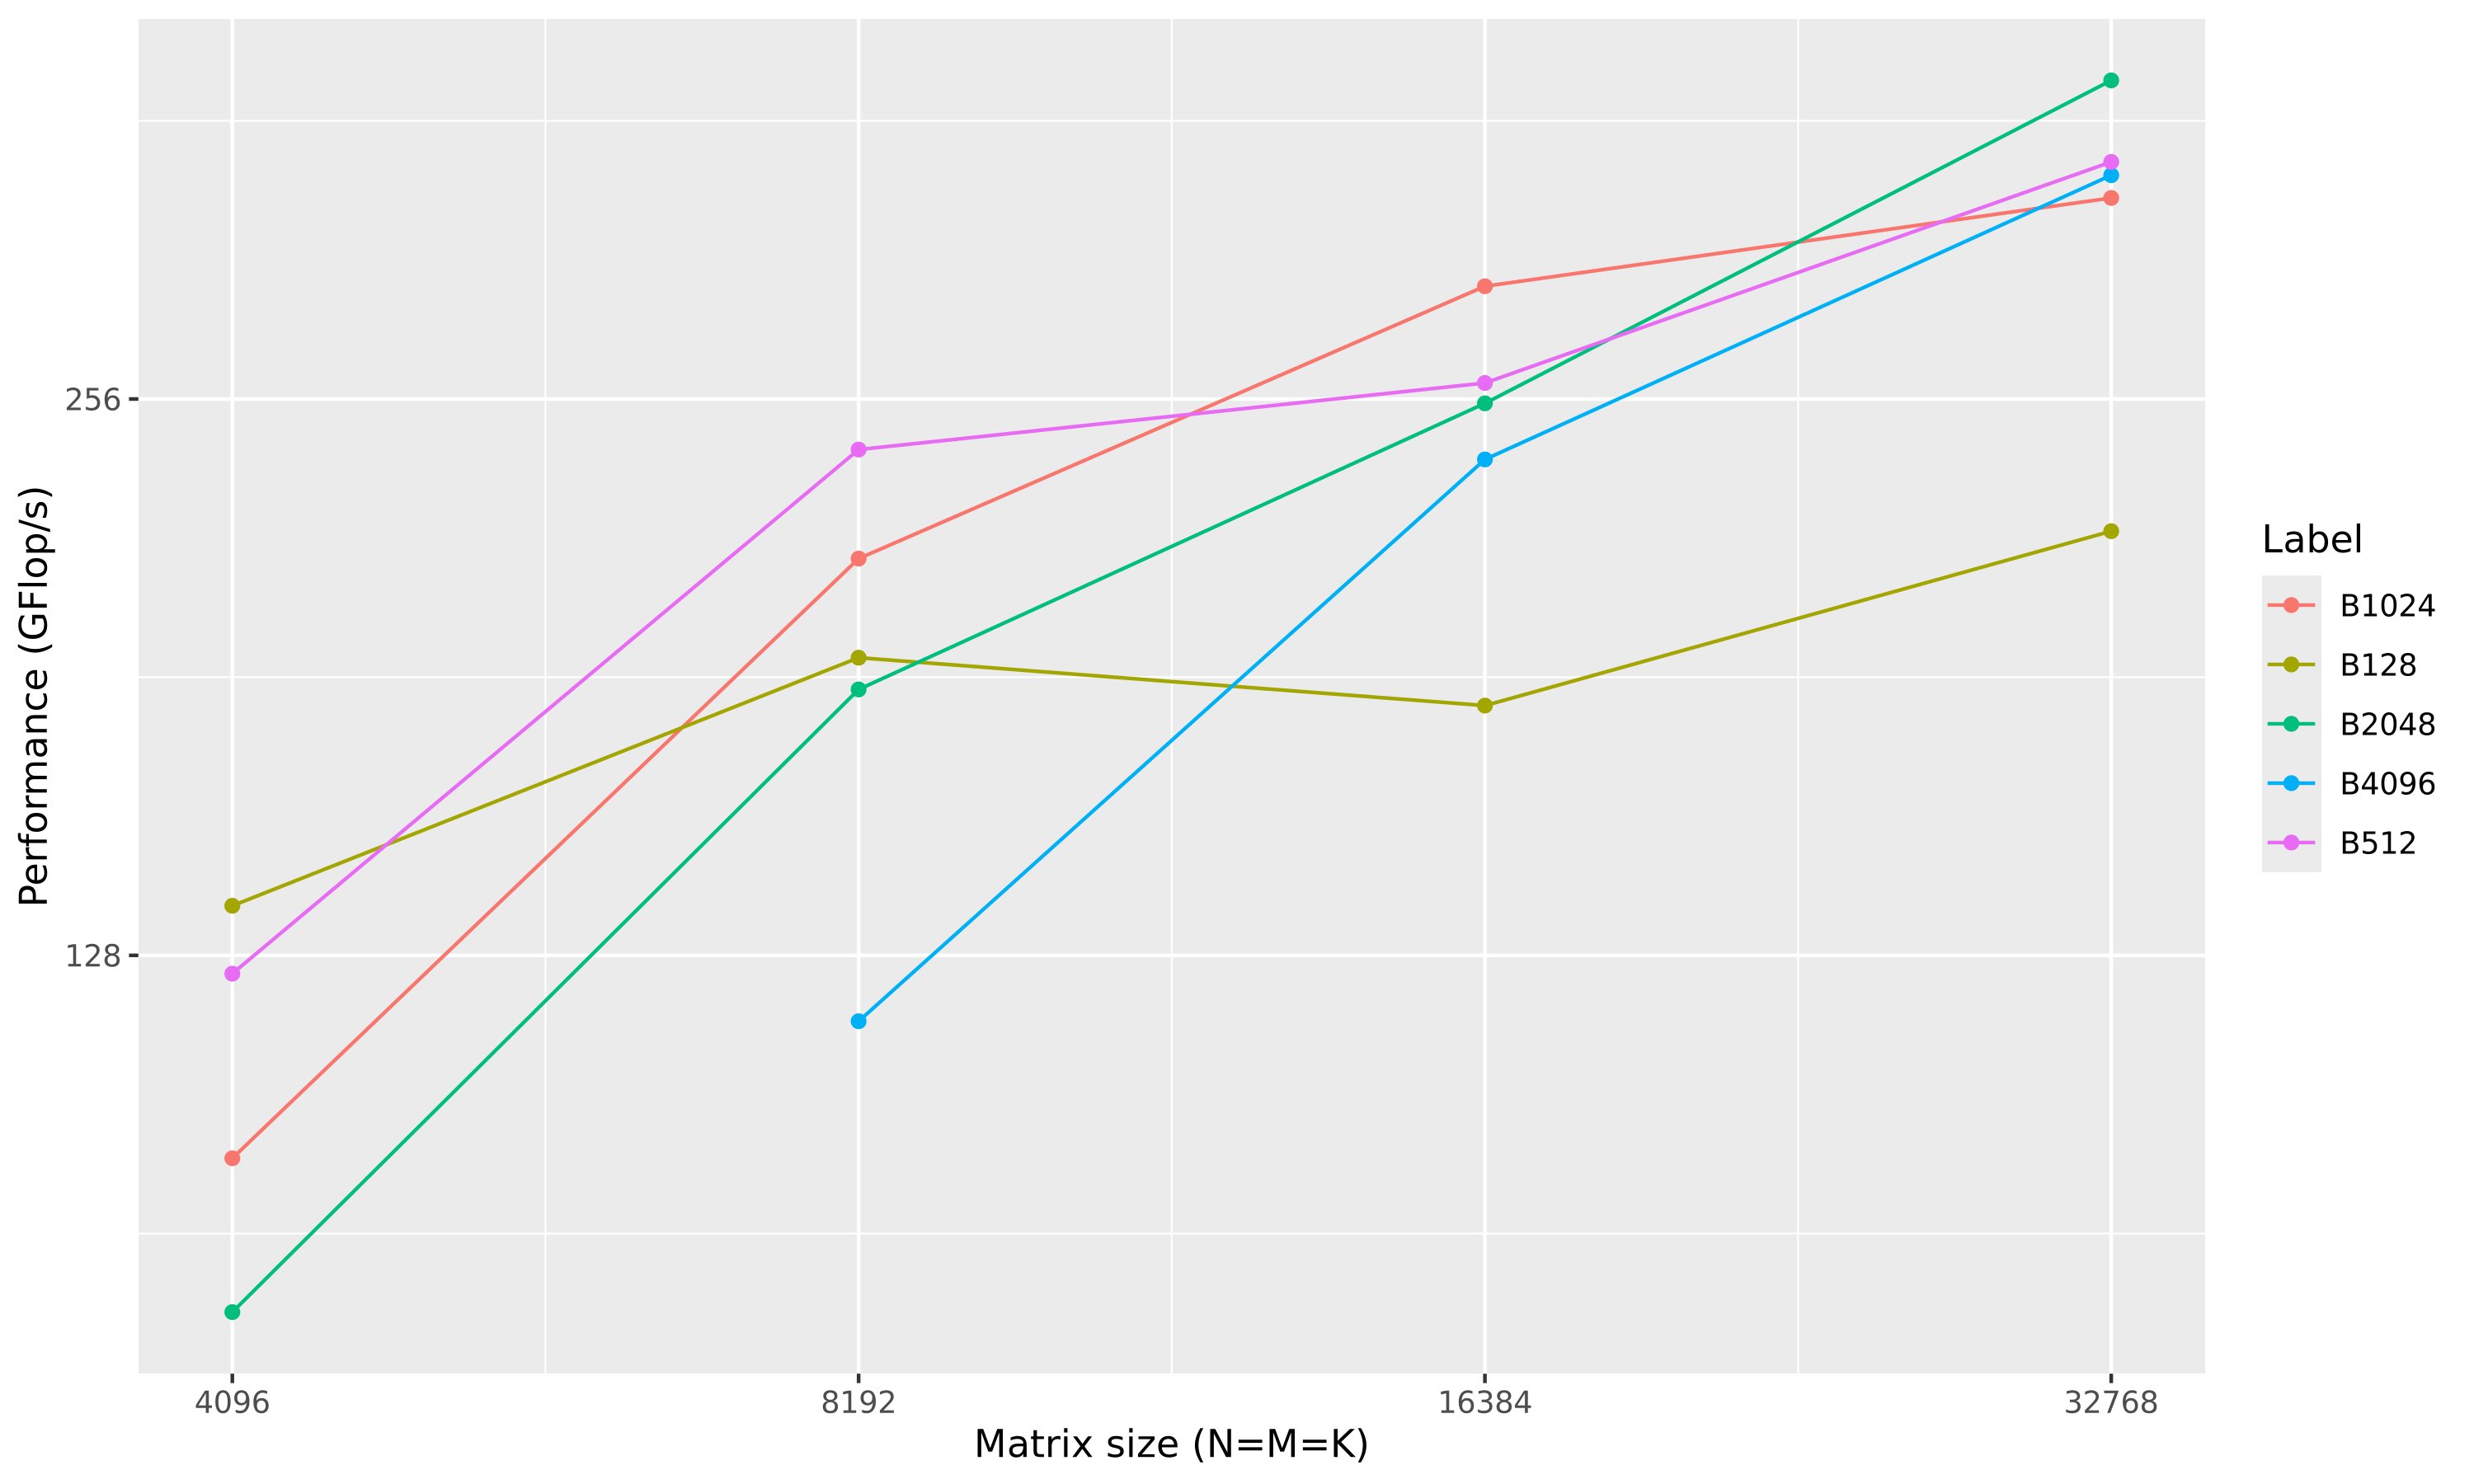
\includegraphics[width=\textwidth]{MPI_block_size.png}
    \caption{Performance depending on set block size}
\end{figure}

\end{frame}

\begin{frame}
\frametitle{Number of nodes}
\begin{figure}
    \centering
    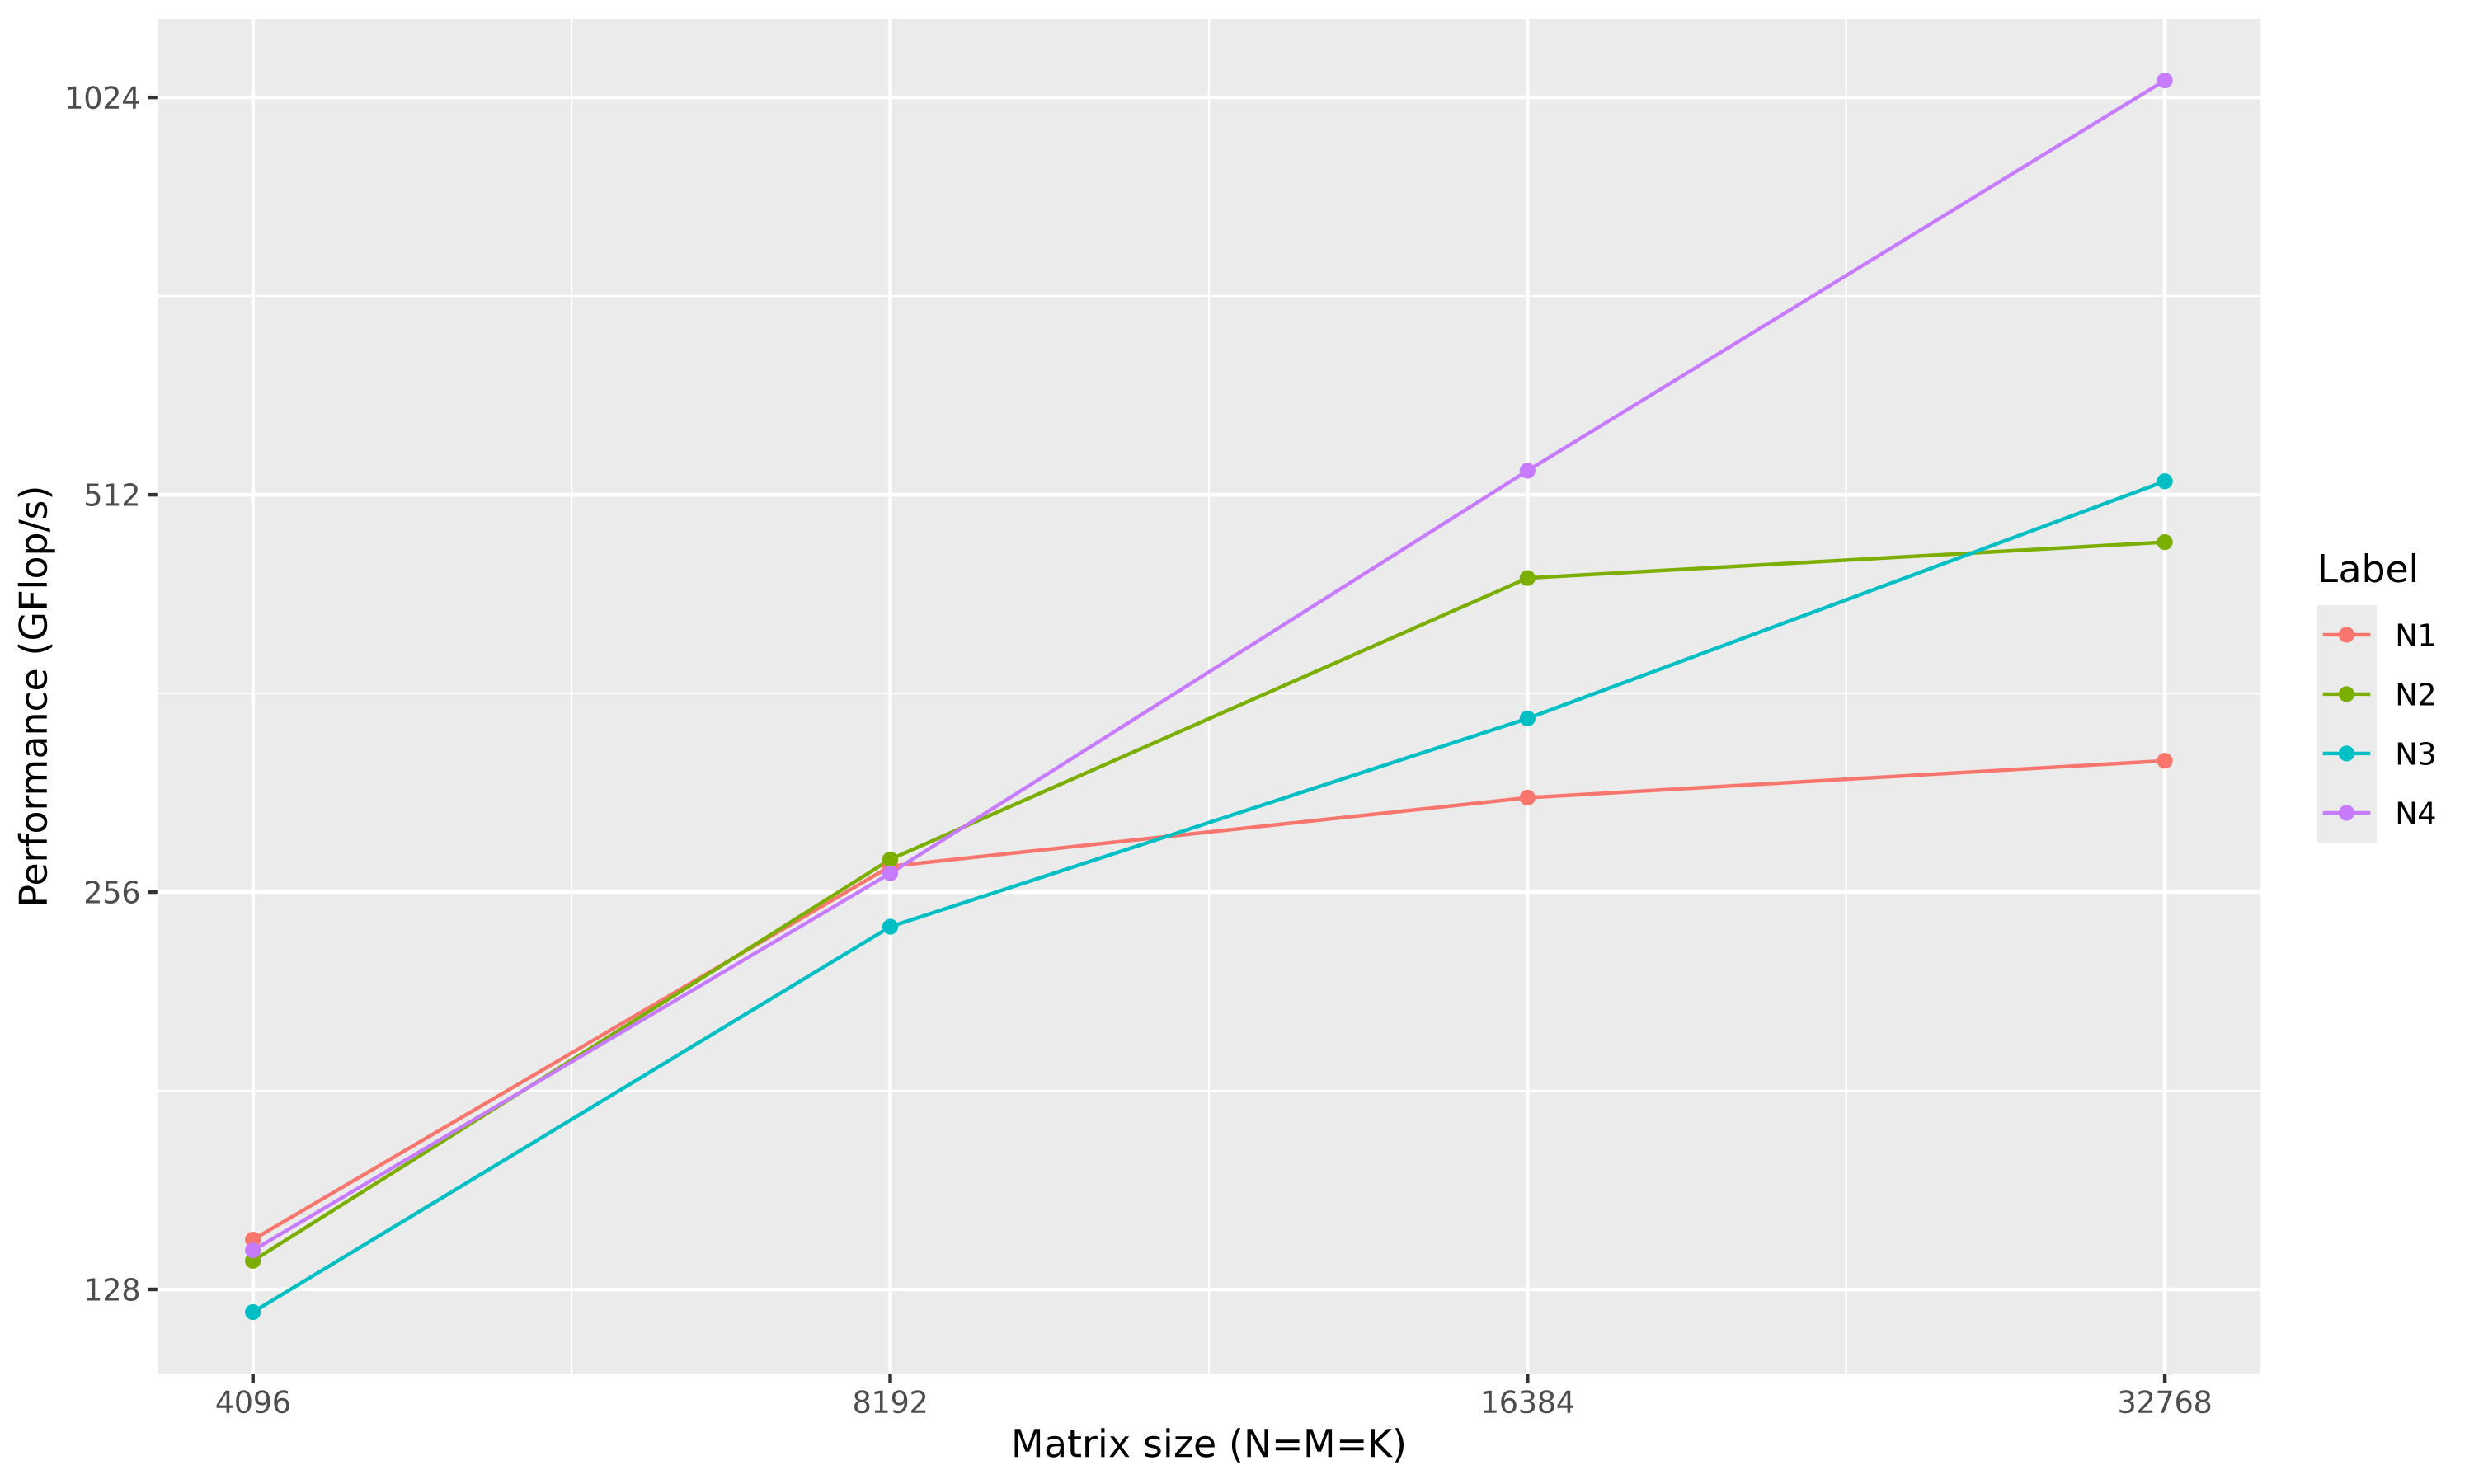
\includegraphics[width=\textwidth]{MPI_nodes.png}
    \caption{Performance depending on number of nodes}
\end{figure}

\end{frame}

\begin{frame}
\frametitle{Enhancements}
\begin{itemize}
    \item Add timers to determine ratio computation/communications
    \item Broadcast could possibly be non-blocking (maybe hard to implement)
    \item Use blocked GEMM 
\end{itemize}
\end{frame}



\end{document}